Figures \ref{ArticleKL-C1880} to \ref{ArticleKL-N1995} show the results for the 3 different years trying to represent the articles with each year :

\begin{figure}[h!]
    \begin{minipage}[b]{0.48\linewidth}
        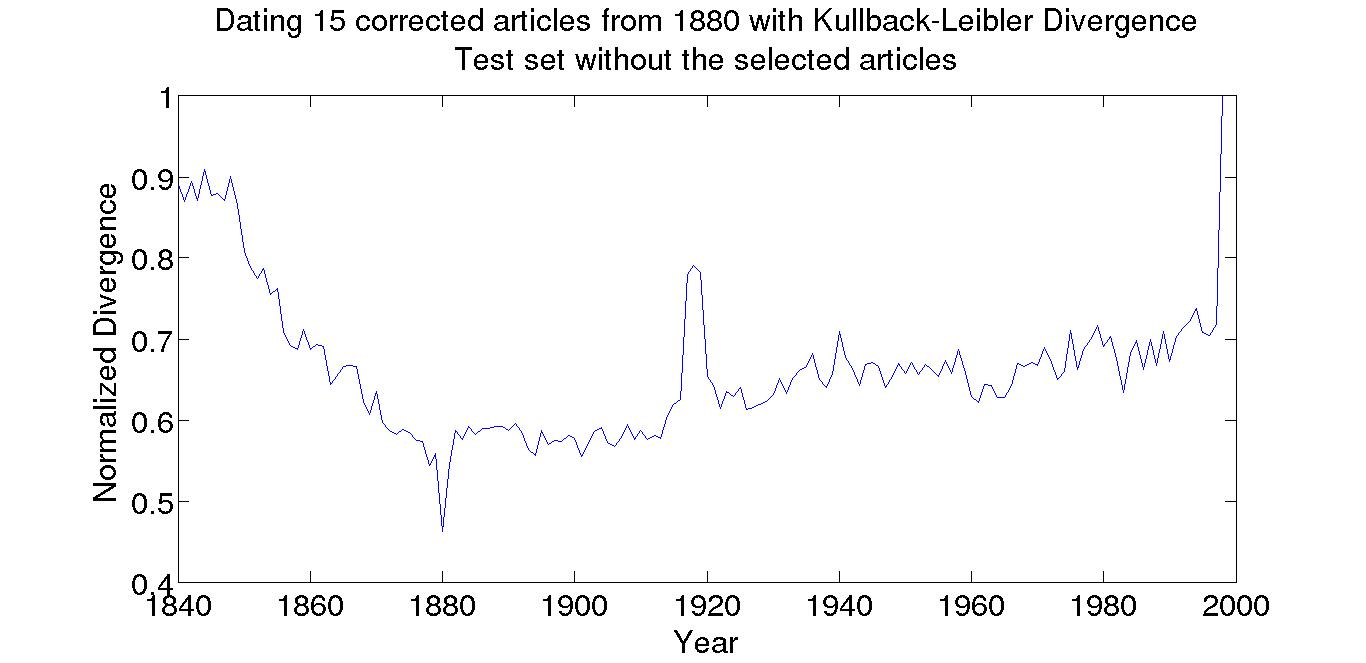
\includegraphics[scale=0.15]{Pictures/date_articles/kullback_leibler/15articles_1880_KL_years_simulate_articles_corrected_without_articles.jpg}
        \caption{KL for 15 articles with OCR correction for year 1880}
        \label{ArticleKL-C1880}
    \end{minipage}\hfill
    \begin{minipage}[b]{0.5\linewidth}
        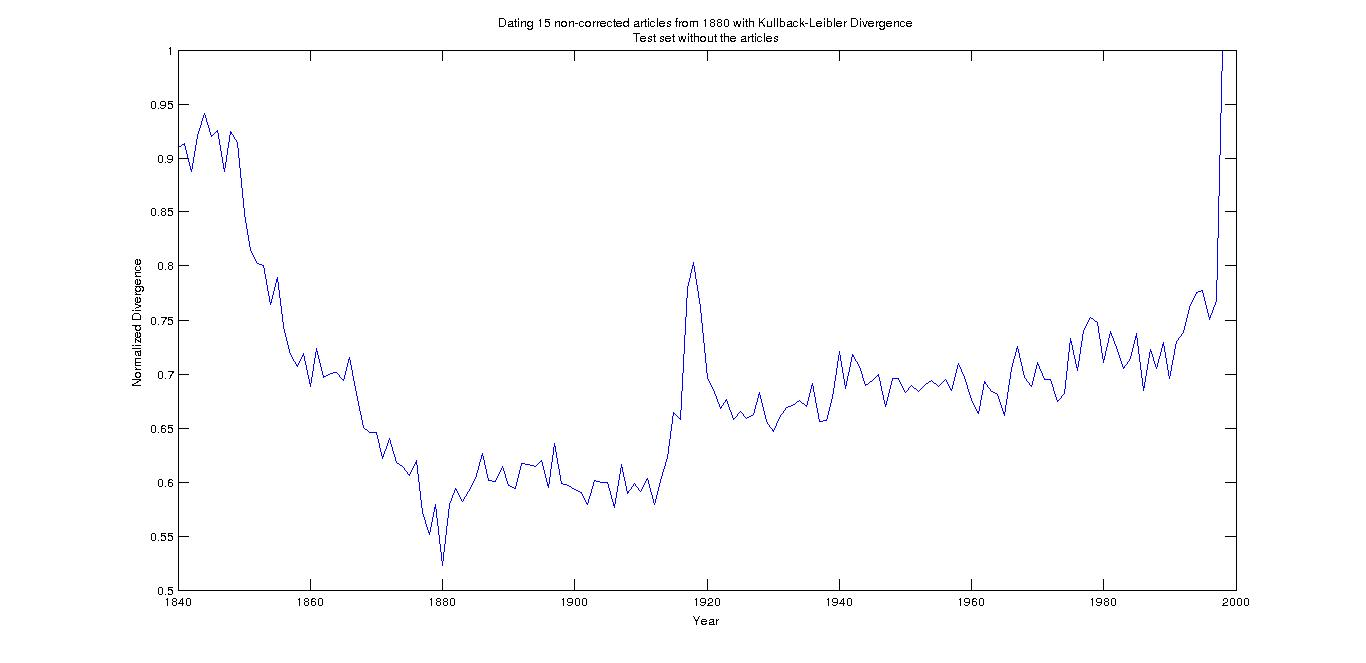
\includegraphics[scale=0.15]{Pictures/date_articles/kullback_leibler/15articles_1880_KL_years_simulate_articles_without_correction_without_articles.jpg}
        \caption{KL for 15 articles without OCR correction for year 1880}
        \label{ArticleKL-N1880}
    \end{minipage}\hfill
\end{figure}

\begin{figure}[h!]
    \begin{minipage}[b]{0.48\linewidth}
        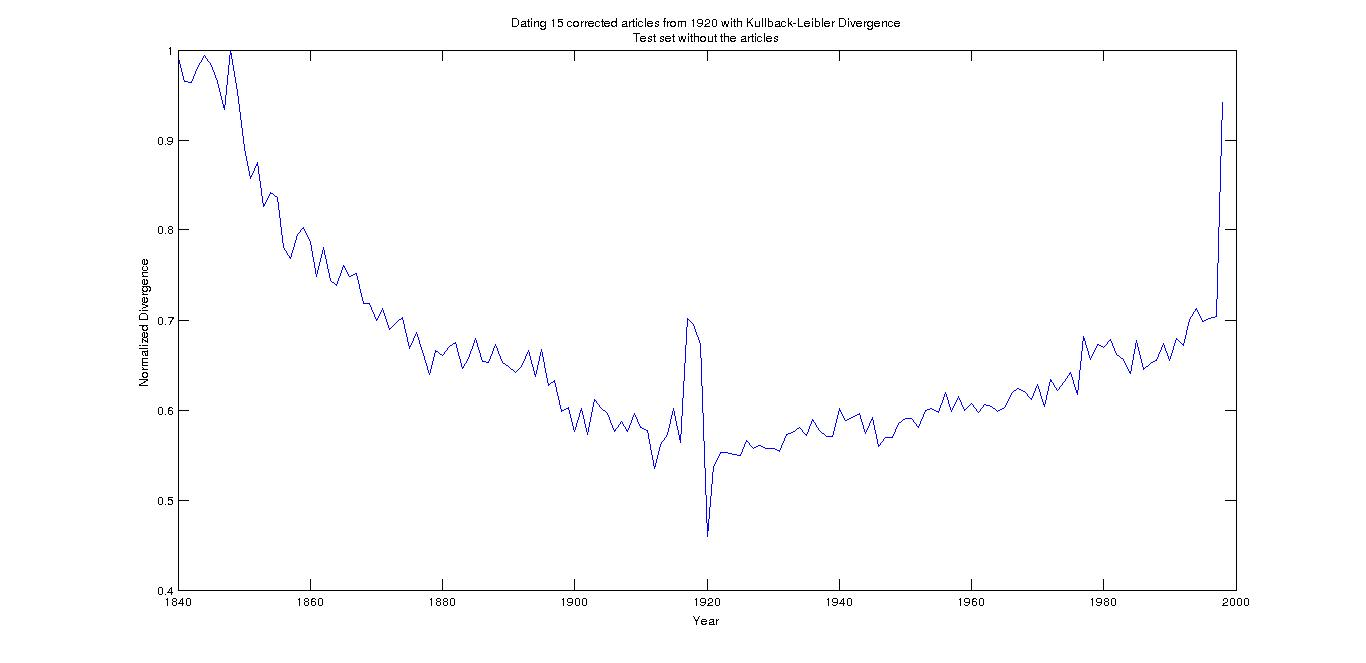
\includegraphics[scale=0.15]{Pictures/date_articles/kullback_leibler/15articles_1920_KL_years_simulate_articles_corrected_without_articles.jpg}
        \caption{KL for 15 articles with OCR correction for year 1920}
        \label{ArticleKL-C1920}
    \end{minipage}\hfill
    \begin{minipage}[b]{0.5\linewidth}
        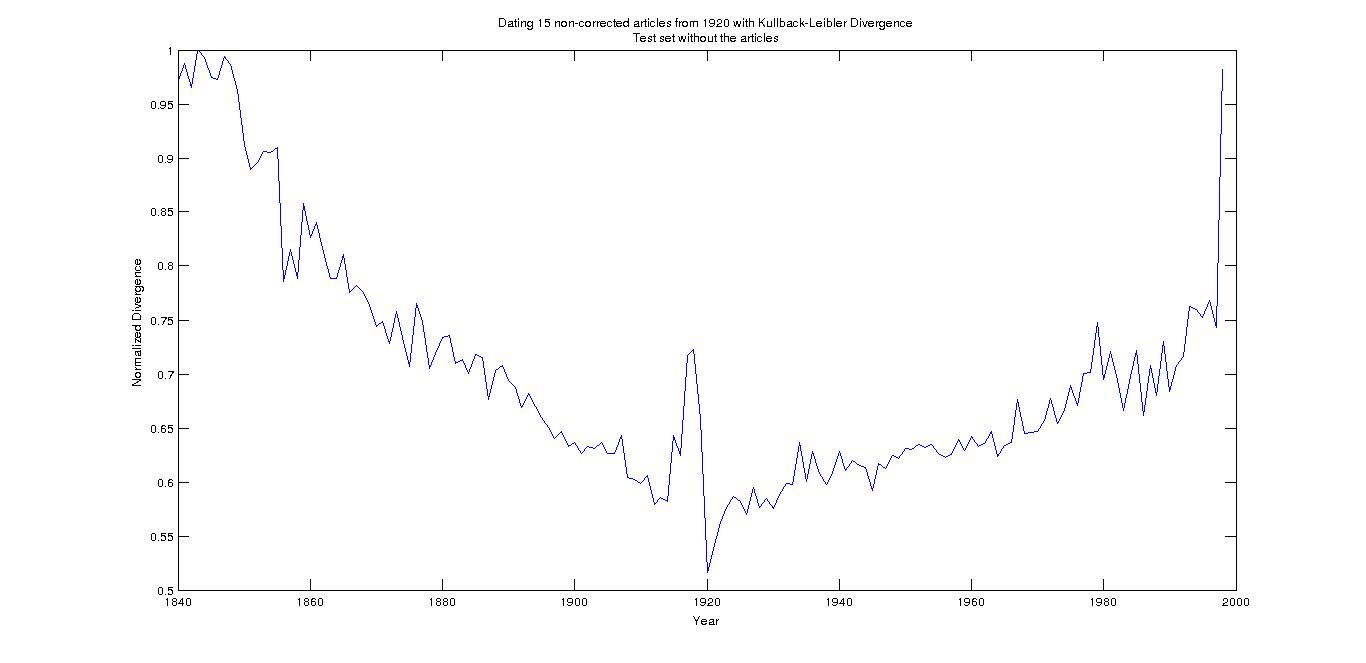
\includegraphics[scale=0.15]{Pictures/date_articles/kullback_leibler/15articles_1920_KL_years_simulate_articles_without_correction_without_articles.jpg}
        \caption{KL for 15 articles without OCR correction for year 1920}
        \label{ArticleKL-N1920}
    \end{minipage}\hfill
\end{figure}

\begin{figure}[h!]
    \begin{minipage}[b]{0.48\linewidth}
        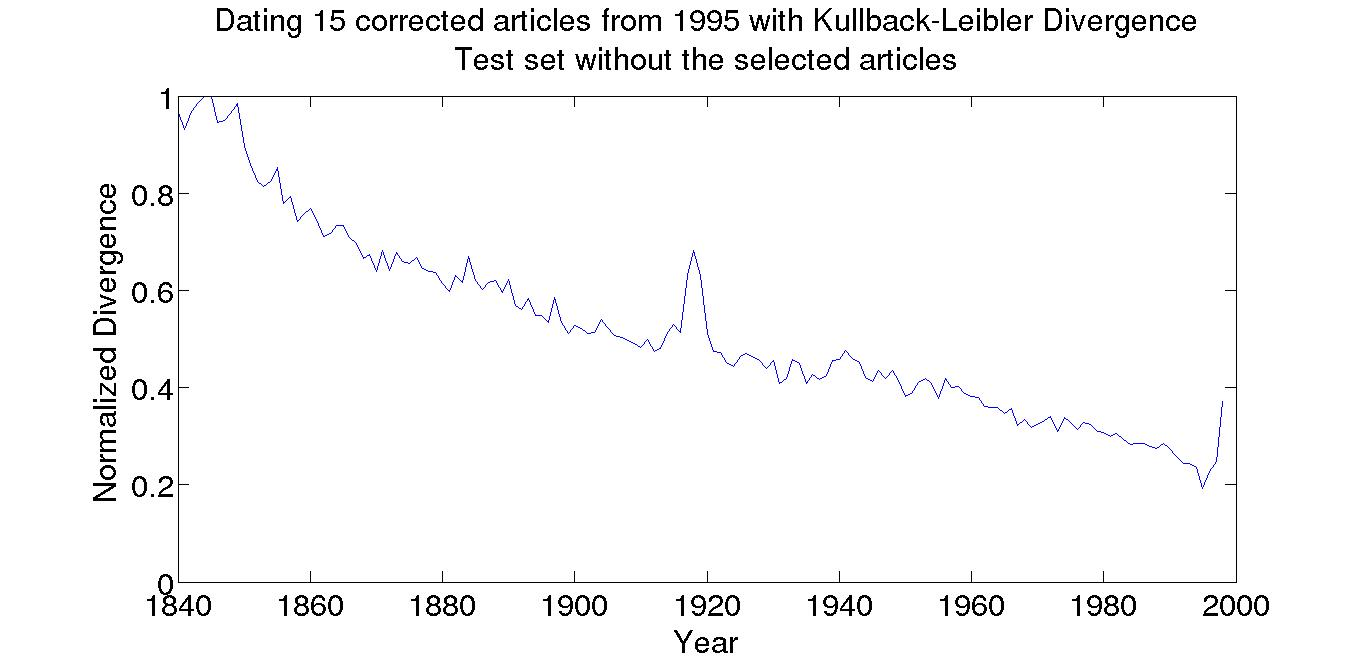
\includegraphics[scale=0.15]{Pictures/date_articles/kullback_leibler/15articles_1995_KL_years_simulate_articles_corrected_without_articles.jpg}
        \caption{KL for 15 articles with OCR correction for year 1995}
        \label{ArticleKL-C1995}
    \end{minipage}\hfill
    \begin{minipage}[b]{0.5\linewidth}
        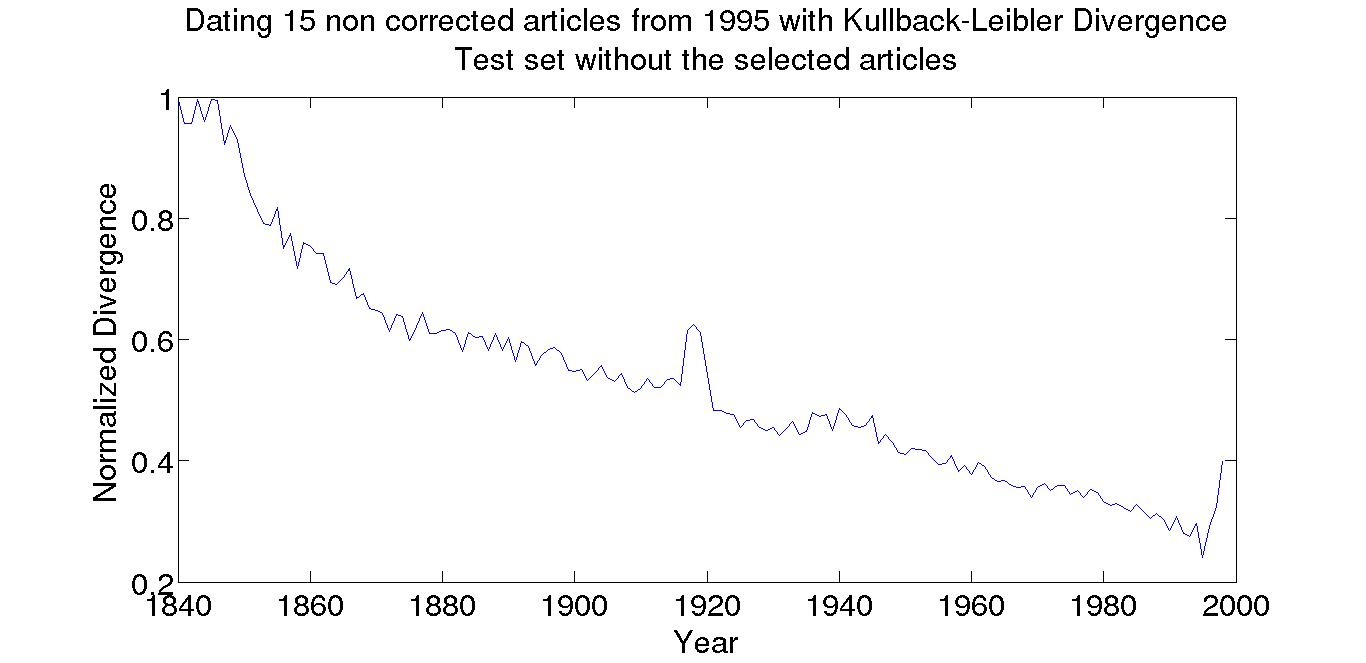
\includegraphics[scale=0.15]{Pictures/date_articles/kullback_leibler/15articles_1995_KL_years_simulate_articles_without_correction_without_articles.jpg}
        \caption{KL for 15 articles without OCR correction for year 1995}
        \label{ArticleKL-N1995}
    \end{minipage}\hfill
\end{figure}

We took only the direction where the year approximate the articles because it has no sense to do the inverse. Indeed, to approximate a year that contains thousands of words with a subset of articles that contains a few hundred words will lead to a dating that will very often predict the years with less words (in the 19$th$ century).

We can observe again in these figures that the OCR correction does not help so much for dating. But, we can observe that the \emph{Kullback-Leibler} Divergence is really good to date the articles. Our explanation for these excellent results is that when we remove some articles from a year, the probability that the words are present in this year is higher than in other years. So, even if we remove the articles from the year, it stays hardly attached to the article and when the year approximate the articles, it has a really good matching.